\documentclass[letterpaper]{article}
\usepackage[submission]{../AAAI_AuthorKit27/aaai2027}
\usepackage[hyphens]{url}
\usepackage{graphicx}
\urlstyle{rm}
\def\UrlFont{\rm}
\usepackage{natbib}
\usepackage{caption}
\frenchspacing
\usepackage{amsmath,amssymb,amsthm}
\usepackage{booktabs}

\newtheorem{theorem}{Theorem}
\newtheorem{lemma}[theorem]{Lemma}
\newtheorem{proposition}[theorem]{Proposition}
\newtheorem{corollary}[theorem]{Corollary}
\newcommand{\E}{\mathbb E}
\newcommand{\R}{\mathcal R}
\newcommand{\cS}{\mathcal S}
\newcommand{\1}{\mathbf 1}

\title{Supplementary Material for\\
When More Epochs Stop Helping: Coverage-Limited Scaling Laws for Sparse Replay}
\author{Anonymous Submission}
\affiliations{}

\begin{document}
\maketitle

\section{Notation and Assumptions}

For coordinate \(j\ge1\),
\[
X_j=q_jZ_jE_j,\qquad
Z_j\sim{\rm Bernoulli}(p_j),\qquad
E_j\sim{\rm Rad},
\]
independently over coordinates and examples.  The covariance is diagonal with
\(\lambda_j=p_jq_j^2\).  Labels are
\(Y=\langle\theta,X\rangle\), and
\(g_j=\lambda_j\theta_j^2\).  There are constants
\(0<c<C<\infty\) such that
\[
\begin{aligned}
cj^{-s}&\le p_j\le Cj^{-s},\\
cj^{-a}&\le\lambda_j\le Cj^{-a},\\
cj^{-b}&\le g_j\le Cj^{-b}.
\end{aligned}
\]
We assume
\[
s>1,\qquad a\ge s,\qquad b>1,\qquad
\sup_jp_j<1,
\]
and that \(\lambda_j\) is nonincreasing up to a constant.  For the coactive
upper bound we additionally assume
\[
a-s+1<b<a+1.
\]
Define
\[
\alpha=\frac{a-b+1}{s},\qquad
\beta=\frac{b-1}{s},
\]
so \(0<\alpha<1\), \(\beta>0\), and
\(\alpha+\beta=a/s\).

Since \(\sum_jp_j<\infty\), the Borel--Cantelli lemma implies that every input
has finite support almost surely.  Thus all inner products below are
well-defined even though the ambient feature set is countably infinite.
For linear predictors, population excess risk is
\[
\R(w)=\sum_j\lambda_j(w_j-\theta_j)^2.
\]
For arbitrary measurable predictors, write
\(\R(f;\theta)=\E_X[(f(X)-\langle\theta,X\rangle)^2]\).

\section{Universal Coverage Lower Bound}

For the lower bound, write
\(\theta_j=\tau_j\Omega_j\), where the magnitudes \(\tau_j\) are fixed and
\(\Omega_j\) are independent Rademacher signs.

\begin{theorem}[Unseen-feature lower bound]
For every measurable, possibly randomized predictor trained on \(n\) unique
examples,
\[
\E_{\Omega,D_n}\R(\widehat f;\theta)
\ge
\sum_{j\ge1}g_j(1-p_j)^n.
\]
\end{theorem}

\begin{proof}
Let
\[
U(D_n)=\{j:Z_{1j}=\cdots=Z_{nj}=0\}
\]
be the set of unseen coordinates.  Conditional on all training inputs, all
teacher signs outside \(U\), and the learner's internal randomness, no
training label depends on \(\{\Omega_j:j\in U\}\).  These signs therefore
remain independent and symmetric.

For an independent test input, define
\[
H(X)=\sum_{j\notin U}\tau_j\Omega_jX_j.
\]
For any finite \(F\subset U\),
\begin{align*}
&\E_{\Omega_F}
\left(
\widehat f(X)-H(X)
-\sum_{j\in F}\tau_j\Omega_jX_j
-\sum_{j\in U\setminus F}\tau_j\Omega_jX_j
\right)^2\\
&\hspace{5mm}\ge
\sum_{j\in F}\tau_j^2X_j^2.
\end{align*}
Equivalently, one can first absorb the coordinates in \(U\setminus F\) into
the term independent of \(\Omega_F\); all cross terms vanish by symmetry.
Let \(F\uparrow U\) and use monotone convergence.  Averaging over the test
input gives at least
\[
\sum_{j\in U}\lambda_j\tau_j^2
=
\sum_{j\in U}g_j.
\]
Finally,
\(\Pr(j\in U)=(1-p_j)^n\), which proves the claim.
\end{proof}

This is a Bayes lower bound under the uniform sign prior and therefore also a
minimax lower bound over deterministic teacher-sign choices.

\begin{lemma}[Power-law occupancy tail]
If \(p_j\asymp j^{-s}\) and \(g_j\asymp j^{-b}\), then
\[
\sum_jg_j(1-p_j)^n\asymp n^{-(b-1)/s}.
\]
For exact \(p_j=c_pj^{-s}\), \(g_j=c_gj^{-b}\), and \(0<c_p<1\),
\[
\sum_jg_j(1-p_j)^n
\sim
\frac{c_g}{s}\Gamma\!\left(\frac{b-1}{s}\right)
(c_pn)^{-(b-1)/s}.
\]
\end{lemma}

\begin{proof}
Let \(J=n^{1/s}\).  For the upper bound,
\((1-p_j)^n\le e^{-np_j}\).  The tail \(j>J\) is
\(O(J^{1-b})\).  On the dyadic shell
\(j\in(J/2^{\ell+1},J/2^\ell]\), the head contributes at most
\[
CJ^{1-b}2^{(b-1)\ell}e^{-c2^{s\ell}}.
\]
The series over \(\ell\) is finite.  For the lower bound, choose a fixed
\(L\) such that \(np_j\le1/2\) for \(j\in[LJ,2LJ]\).  Bernoulli's inequality
gives \((1-p_j)^n\ge1-np_j\ge1/2\), and that shell contributes
\(\Omega(J^{1-b})\).

For the sharp constant, set \(J=(c_pn)^{1/s}\).  Uniformly on the relevant
scale,
\[
(1-c_pj^{-s})^n\to e^{-(J/j)^s}.
\]
A Riemann-sum argument, with the preceding head and tail bounds providing
domination, gives
\[
J^{b-1}\sum_jj^{-b}(1-c_pj^{-s})^n
\longrightarrow
\int_0^\infty u^{-b}e^{-u^{-s}}\,du.
\]
The substitution \(t=u^{-s}\) evaluates the integral as
\[
\frac1s\Gamma\!\left(\frac{b-1}{s}\right).
\]
Multiplying by \(c_gJ^{1-b}\) proves the result.
\end{proof}

\section{Exact One-Hot Replay}

Suppose each example chooses one coordinate
\(J_i\sim(p_j)\) and equals
\(X_i=E_iq_{J_i}e_{J_i}\).  Let
\(C_j=\sum_{i=1}^n\1\{J_i=j\}\).

\begin{proposition}[Exact finite-epoch risk]
Train a width-\(m\) model from zero by squared-loss SGD with step size \(\eta\)
for \(K\) repeated passes over the same dataset.  Then
\[
\R_D
=
\sum_{j\le m}g_j(1-\eta q_j^2)^{2KC_j}
+\sum_{j>m}g_j,
\]
and
\[
\E_D\R_D
=
\sum_{j\le m}g_j
[1-p_j+p_j(1-\eta q_j^2)^{2K}]^n
+\sum_{j>m}g_j.
\]
\end{proposition}

\begin{proof}
Let \(\delta_j=w_j-\theta_j\).  An example supported on \(j\) gives
\[
\delta_j^+=(1-\eta q_j^2)\delta_j.
\]
Coordinate updates commute, and coordinate \(j\) is updated \(KC_j\) times.
The first expression follows from diagonal population risk.  Since
\(C_j\sim{\rm Binomial}(n,p_j)\), the second follows from the binomial
probability-generating function.
\end{proof}

\begin{theorem}[Three-frontier law]
Assume \(\sup_jp_j\le\bar p<1\) and
\(0<\eta q_j^2\le\rho<1\).  Let
\[
J_\star=\min\{m,(\eta nK)^{1/a},n^{1/s}\}.
\]
Then
\[
\E_D\R_D\asymp J_\star^{1-b}.
\]
Equivalently,
\[
\E_D\R_D
\asymp
m^{-(b-1)}
+(\eta nK)^{-(b-1)/a}
+n^{-(b-1)/s}.
\]
\end{theorem}

\begin{proof}
Set \(\xi_j=\eta q_j^2\) and
\[
r_j=1-(1-\xi_j)^{2K}.
\]
Uniformly for \(0<\xi_j\le\rho<1\),
\[
r_j\asymp\min\{1,K\xi_j\}.
\]
Thus
\[
np_jr_j
\asymp
\min\{np_j,\eta nKp_jq_j^2\}
\asymp
\min\{nj^{-s},\eta nKj^{-a}\}.
\]
The exact survival factor is
\((1-p_jr_j)^n\).  Since \(p_jr_j\le\bar p\), it is bounded above and below
by exponentials with constant multiples of \(np_jr_j\) in the exponent.

Write \(A=\eta nK\), \(B=n\), and
\(J=\min\{m,A^{1/a},B^{1/s}\}\).  It remains to bound
\[
S=
\sum_{j\le m}j^{-b}
e^{-c\min\{Aj^{-a},Bj^{-s}\}}
+\sum_{j>m}j^{-b}.
\]
For \(j\le J\), \(A\ge J^a\) and \(B\ge J^s\), so, using \(a\ge s\),
\[
\min\{Aj^{-a},Bj^{-s}\}
\ge
\min\{(J/j)^a,(J/j)^s\}
=
(J/j)^s.
\]
The dyadic-shell argument from the occupancy lemma bounds the core by
\(O(J^{1-b})\); all indices above \(J\) contribute at most the same order.

For the lower bound, if \(J=m\), the omitted tail is
\(\Omega(J^{1-b})\).  Otherwise, either \(m<2J\), in which case the omitted
tail again suffices, or the represented shell \([J,2J]\) has exponent bounded
by a constant and contributes \(\Omega(J^{1-b})\).
\end{proof}

\section{Occupancy and Source Lemmas for Coactive Data}

For \(N\) selected examples, define
\[
\cS_N=\bigcup_{i=1}^N{\rm supp}(X_i),\qquad
V_N=|\cS_N|,\qquad
A_N=\sum_{j\in\cS_N}\theta_j^2.
\]

\begin{lemma}[Singleton anchors]
Let
\[
\pi_0=\prod_{k\ge1}(1-p_k).
\]
Then \(\pi_0>0\), and the probability that one example has support exactly
\(\{j\}\) is
\[
\nu_j
=
p_j\prod_{k\ne j}(1-p_k)
=
\frac{\pi_0p_j}{1-p_j}
\asymp p_j.
\]
For every \(r>0\), there is \(c_J>0\) such that, with
\[
J_N=\left\lfloor
c_J\left(\frac{N}{\log(eN)}\right)^{1/s}
\right\rfloor,
\]
\[
\Pr\left(
C_{N,j}\ge c_0Np_j\text{ for all }j\le J_N
\right)\ge1-N^{-r},
\]
where \(C_{N,j}\) counts singleton-\(j\) examples.
\end{lemma}

\begin{proof}
The product is positive because \(\sum_jp_j<\infty\) and
\(\sup_jp_j<1\).  For fixed \(j\),
\(C_{N,j}\sim{\rm Binomial}(N,\nu_j)\).  If \(j\le J_N\), then
\[
N\nu_j\ge cc_J^{-s}\log(eN).
\]
The multiplicative Chernoff inequality gives
\[
\Pr(C_{N,j}<N\nu_j/2)\le e^{-N\nu_j/8}.
\]
Choose \(c_J\) so the right side is at most \(N^{-(r+2)}\), and union bound
over at most \(N\) indices.  Since \(\nu_j\asymp p_j\), the stated constant
\(c_0\) follows.
\end{proof}

\begin{lemma}[Observed dictionary size]
The indicators \(I_{N,j}=\1\{j\in\cS_N\}\) are independent and
\[
\E V_N
=
\sum_j[1-(1-p_j)^N]
\asymp N^{1/s}.
\]
For exact \(p_j=c_pj^{-s}\),
\[
\E V_N
\sim
\Gamma(1-1/s)(c_pN)^{1/s}.
\]
There is \(c_m>0\) such that \(N\le c_mm^s\) implies
\[
\Pr(V_N>m)\le e^{-cm}.
\]
\end{lemma}

\begin{proof}
Each \(I_{N,j}\) is a function only of
\(\{Z_{ij}\}_{i=1}^N\), so the indicators are independent across \(j\).
Also
\[
\E I_{N,j}=1-(1-p_j)^N\asymp\min\{1,Np_j\}.
\]
Splitting at \(N^{1/s}\) proves the order.  For the exact constant, with
\(J=(c_pN)^{1/s}\),
\[
\begin{aligned}
&J^{-1}\sum_j[1-(1-c_pj^{-s})^N]\\
&\qquad\longrightarrow
\int_0^\infty(1-e^{-u^{-s}})\,du
=
\Gamma(1-1/s).
\end{aligned}
\]
Choose \(c_m\) so that \(N\le c_mm^s\) implies
\(\E V_N\le m/2\), then apply a multiplicative Chernoff bound.  Infinite
sums are handled by finite truncation and monotone convergence.
\end{proof}

\begin{lemma}[Observed source norm]
Under \(a-s+1<b<a+1\),
\[
\E A_N
=
\sum_j\theta_j^2[1-(1-p_j)^N]
\asymp N^\alpha,
\qquad
\alpha=\frac{a-b+1}{s}.
\]
For exact
\(p_j=c_pj^{-s}\), \(\lambda_j=c_\lambda j^{-a}\), and
\(g_j=c_gj^{-b}\),
\[
\E A_N
\sim
\frac{c_g}{c_\lambda}
\frac{\Gamma(1-\alpha)}{a-b+1}
(c_pN)^\alpha.
\]
\end{lemma}

\begin{proof}
Because \(\theta_j^2=g_j/\lambda_j\asymp j^{a-b}\), set
\(J=N^{1/s}\) and split:
\[
\sum_{j\le J}j^{a-b}
\asymp J^{a-b+1},
\]
using \(b<a+1\), while
\[
N\sum_{j>J}j^{a-b-s}
\asymp NJ^{a-b-s+1},
\]
using \(b>a-s+1\).  Both equal \(N^\alpha\).

For exact profiles, rescaling by \(J=(c_pN)^{1/s}\) gives the integral
\[
\int_0^\infty
u^{a-b}(1-e^{-u^{-s}})\,du.
\]
Letting \(t=u^{-s}\) and integrating by parts,
\[
\int_0^\infty
u^{a-b}(1-e^{-u^{-s}})\,du
=
\frac{\Gamma(1-\alpha)}{a-b+1}.
\]
\end{proof}

\section{Coactive Clipped Replay}

Let the selected dictionary contain all features in \(\cS_N\), assuming
\(V_N\le m\).  At update \(t\), sample \(I_t\) uniformly from
\(\{1,\ldots,N\}\), set
\[
\gamma_i
=
\min\left\{\eta,\frac{\rho}{\|X_i\|^2}\right\},
\qquad0<\rho\le1,
\]
where the second argument is interpreted as \(+\infty\) for a zero row.
and update
\[
w_{t+1}
=
w_t-\gamma_{I_t}X_{I_t}
(X_{I_t}^\top w_t-Y_{I_t}).
\]
Assume
\(\eta\sup_jq_j^2\le\rho\), and output
\[
\bar w_T=\frac1T\sum_{t=0}^{T-1}w_t.
\]

Define the observable good event
\[
\mathcal G_N
=
\{V_N\le m\}
\cap
\{C_{N,j}\ge c_0Np_j\text{ for every }j\le J_N\}.
\]
The support-certified algorithm returns zero if this event fails.

\begin{lemma}[Pathwise contraction]
Let \(\delta_t=w_t-\theta_{\cS_N}\).  Every update satisfies
\[
\|\delta_{t+1}\|^2
\le
\|\delta_t\|^2-\gamma_{I_t}
(X_{I_t}^\top\delta_t)^2.
\]
In particular,
\[
\|\delta_t\|\le\|\delta_0\|=\sqrt{A_N}
\]
for every update path.
\end{lemma}

\begin{proof}
For a row \(x\),
\[
\delta^+=(I-\gamma xx^\top)\delta.
\]
Therefore
\[
\|\delta^+\|^2
=
\|\delta\|^2
-\gamma(2-\gamma\|x\|^2)(x^\top\delta)^2.
\]
By construction, \(\gamma\|x\|^2\le\rho\le1\), so
\(2-\gamma\|x\|^2\ge1\).
\end{proof}

\begin{lemma}[Certified curvature]
Condition on \(D_N\in\mathcal G_N\).  Then
\[
\E_t\|\delta_{t+1}\|^2
\le
\|\delta_t\|^2
-c\eta\sum_{j\le J_N}\lambda_j\delta_{t,j}^2.
\]
\end{lemma}

\begin{proof}
Average the contraction inequality over a uniform choice among the \(N\)
training rows.  All contributions are nonnegative, so retain only singleton
rows.  A singleton-\(j\) row is \(\pm q_je_j\).  It is not clipped because
\(\eta q_j^2\le\rho\), and therefore contributes
\(\eta q_j^2\delta_j^2\).  Consequently,
\[
\frac1N\sum_{i=1}^N
\gamma_i(X_i^\top\delta)^2
\ge
\frac\eta N\sum_{j\le J_N}
C_{N,j}q_j^2\delta_j^2.
\]
On \(\mathcal G_N\),
\(C_{N,j}\ge c_0Np_j\), and
\(p_jq_j^2=\lambda_j\).
\end{proof}

\begin{theorem}[Conditional coactive replay bound]
Condition on \(D_N\in\mathcal G_N\).  Then
\[
\E_{\rm sgd}\R(\bar w_T)
\le
\frac{A_N}{c\eta T}
+C\lambda_{J_N+1}A_N
+\sum_{j\notin\cS_N}g_j.
\]
\end{theorem}

\begin{proof}
Telescope the certified-curvature inequality:
\[
c\eta
\sum_{t=0}^{T-1}
\E_{\rm sgd}
\sum_{j\le J_N}\lambda_j\delta_{t,j}^2
\le
\|\delta_0\|^2=A_N.
\]
Jensen's inequality gives
\[
\E_{\rm sgd}
\sum_{j\le J_N}\lambda_j\bar\delta_{T,j}^2
\le
\frac{A_N}{c\eta T}.
\]
Pathwise contraction implies
\[
\|\bar\delta_T\|
\le
\frac1T\sum_{t<T}\|\delta_t\|
\le\sqrt{A_N}.
\]
Since the spectrum is nonincreasing up to constants,
\[
\sum_{\substack{j>J_N\\j\in\cS_N}}
\lambda_j\bar\delta_{T,j}^2
\le
C\lambda_{J_N+1}A_N.
\]
The predictor is zero outside \(\cS_N\), whose exact risk contribution is
\(\sum_{j\notin\cS_N}g_j\).
\end{proof}

\begin{theorem}[Expected coactive replay bound]
Fix \(r>\beta\), choose \(c_J\) for failure exponent \(r\), and suppose
\(N\le c_mm^s\).  The support-certified algorithm satisfies
\[
\E\R(\bar w_T)
\le
C\left[
\frac{N^\alpha}{\eta T}
+\{\log(eN)\}^{a/s}N^{-\beta}
+N^{-r}+e^{-cm}
\right].
\]
\end{theorem}

\begin{proof}
On \(\mathcal G_N\), average the conditional bound over the dataset.
The observed-source lemma gives
\[
\E A_N\lesssim N^\alpha.
\]
Moreover,
\[
\lambda_{J_N+1}\E A_N
\lesssim
\left(\frac{N}{\log(eN)}\right)^{-a/s}N^\alpha
=
\{\log(eN)\}^{a/s}N^{-\beta},
\]
because \(\alpha+\beta=a/s\).  The unseen-feature lemma contributes
\(O(N^{-\beta})\).

On \(\mathcal G_N^c\), the certified algorithm outputs zero, whose risk is
\(\sum_jg_j<\infty\).  The singleton and dictionary lemmas give
\[
\Pr(\mathcal G_N^c)\le N^{-r}+e^{-cm}.
\]
\end{proof}

\begin{corollary}[All-data saturation]
Set \(N=n\), \(T=nK\), and \(m\gtrsim n^{1/s}\).  Then
\[
\E\R(\bar w_{nK})
\lesssim
\frac{n^{\alpha-1}}{\eta K}
+\{\log(en)\}^{a/s}n^{-\beta}.
\]
Thus
\[
K=\widetilde O(\eta^{-1}n^{a/s-1})
\]
suffices to reach the coverage floor up to logarithms.
\end{corollary}

\begin{corollary}[Frontier-matched schedule]
Let
\[
J_\star=\min\{m,n^{1/s},(\eta T)^{1/a}\}
\]
and select
\[
N_\star=
\left\lfloor
c\min\{n,m^s,(\eta T)^{s/a}\}
\right\rfloor
\]
unique examples.  Then, for \(J_\star\) larger than a fixed constant,
\[
\E\R(\bar w_T)
\le
C\{\log(eJ_\star)\}^{a/s}J_\star^{1-b}.
\]
Equivalently,
\[
\E\R(\bar w_T)
=
\widetilde O\left(
m^{-(b-1)}
+(\eta T)^{-(b-1)/a}
+n^{-(b-1)/s}
\right).
\]
\end{corollary}

\begin{proof}
The choice of \(N_\star\) guarantees both
\(N_\star\lesssim m^s\) and
\(\eta T\gtrsim N_\star^{a/s}\).  Hence
\[
\frac{N_\star^\alpha}{\eta T}
\lesssim
N_\star^{\alpha-a/s}
=
N_\star^{-\beta}.
\]
The logarithmic term has the same power.  Finally
\(N_\star^{1/s}\asymp J_\star\), so
\(N_\star^{-\beta}=J_\star^{1-b}\).  Since \(1-b<0\), the largest of the
three frontier terms is equivalent within a factor three to their sum.
\end{proof}

\section{Additional Experimental Details}

\paragraph{Generation.}
For ambient dimension \(d\), we use
\[
p_j=\frac{\mu}{\zeta(s)}j^{-s},\qquad
\lambda_j=j^{-a},\qquad
q_j^2=\frac{\lambda_j}{p_j},\qquad
g_j=j^{-b}.
\]
Teacher signs are independent Rademacher variables.  We draw each coordinate's
occupancy as a binomial random variable and then choose that many rows without
replacement.  This generates the independent Bernoulli design exactly while
using \(O(d+{\rm nnz})\) rather than \(O(nd)\) memory.

Risk within the first \(d\) coordinates is computed exactly from the
coefficient error.  We add the analytic unrepresented tail
\(\zeta(b,d+1)\).  The unseen-feature floor is
\[
\sum_{j\le d}g_j(1-p_j)^n+\zeta(b,d+1).
\]

\paragraph{Optimization.}
The primary method samples with replacement and uses
\[
\gamma_i=\min\{\eta,0.9/\|X_i\|^2\}.
\]
We record both the last iterate and the uniform average of all pre-update
iterates.  Cyclic and independently reshuffled protocols are used as
robustness checks.  No support certificate is applied in any experiment.

\paragraph{Default sweep.}
We use
\[
(s,a,b,\mu,\eta)=(1.5,2,2,1,0.2),
\]
\(d=4096\),
\(n\in\{256,512,\ldots,8192\}\), and
\(K\in\{1,2,\ldots,512\}\), with five seeds.  The fitted two-term law for the
averaged iterate is
\[
0.916(\eta nK)^{-1/2}+1.125n^{-2/3},
\]
with \(R^2=0.9805\) and median relative error \(0.0954\).
For the last iterate, \(R^2=0.9759\) with median relative error \(0.0997\).

\paragraph{Progressive schedule.}
For \(T=2^{12},\ldots,2^{20}\), choose
\(N=\lfloor(\eta T)^{s/a}\rfloor\), \(K=\lfloor T/N\rfloor\),
and \(d=8192\).  The fitted slopes are \(-0.5016\) for the averaged iterate
and \(-0.4970\) for the last iterate, versus the prediction \(-0.5\).

\paragraph{Fixed compute.}
At \(T=2^{18}\), we vary
\(N\in\{256,512,\ldots,32768\}\) and set \(K=T/N\).  Last-iterate risk falls
from \(0.04302\) to \(0.00335\), a factor \(12.84\), as the unique-data
fraction increases.

\paragraph{Source sweep.}
At \((a,s)=(2,1.5)\), \(K=512\), and \(d=8192\), the measured averaged-risk
coverage slopes for
\(b=(1.4,1.7,2.0,2.4)\) are
\((-0.2633,-0.4580,-0.6532,-0.9150)\), compared with
\((-0.2667,-0.4667,-0.6667,-0.9333)\).

\paragraph{Spectrum-grid robustness.}
We additionally test
\((a,s,b)=(2,1.5,2),(2.4,1.5,2),(2.5,2,2.5)\).
Fixed-exponent two-term fits have averaged-risk
\(R^2=(0.989,0.996,0.993)\).  The measured optimization slopes are
\((-0.457,-0.403,-0.545)\), versus
\((-0.500,-0.417,-0.600)\); measured coverage slopes are
\((-0.656,-0.613,-0.788)\), versus
\((-0.667,-0.667,-0.750)\).

\paragraph{Clipping stress test.}
We sweep
\(\mu\in\{1,1.75,2.25\}\) and
\(\eta\in\{0.2,0.4,0.8,1.2\}\).
At \((\mu,\eta)=(2.25,1.2)\), unclipped reshuffling reaches mean risk
\(1.16\times10^{85}\) by epoch four and subsequently overflows.  Clipping
reaches \(0.00708\) by epoch 64; the coverage floor is \(0.00618\).

\begin{figure}[t]
\centering
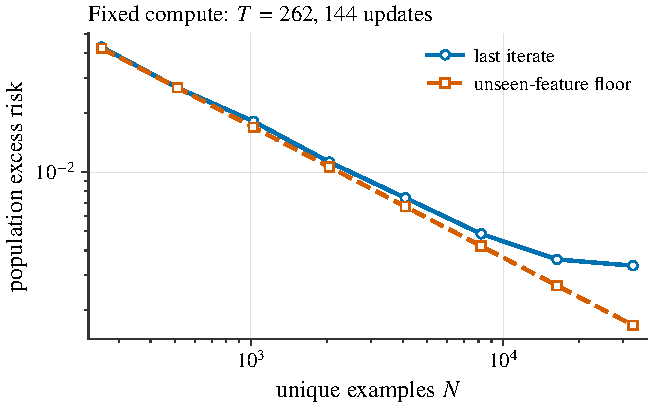
\includegraphics[width=\columnwidth]{figures/fixed_compute.pdf}
\caption{At fixed total updates, more unique data lowers the coverage floor
and improves the final risk.}
\end{figure}

\begin{figure}[t]
\centering
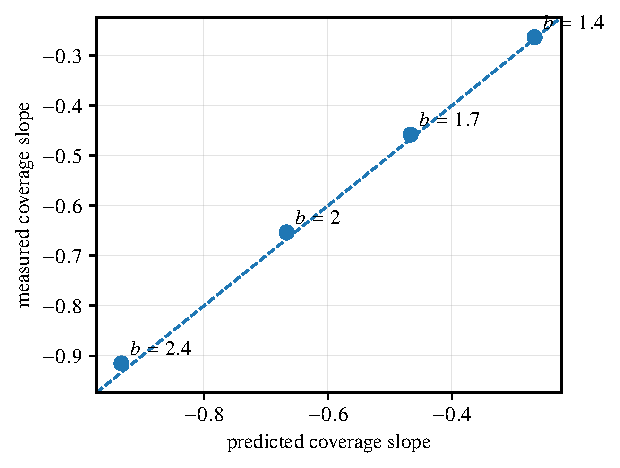
\includegraphics[width=\columnwidth]{figures/source_exponents.pdf}
\caption{Predicted versus measured coverage slopes as the source exponent
\(b\) varies.}
\end{figure}

\begin{figure}[t]
\centering
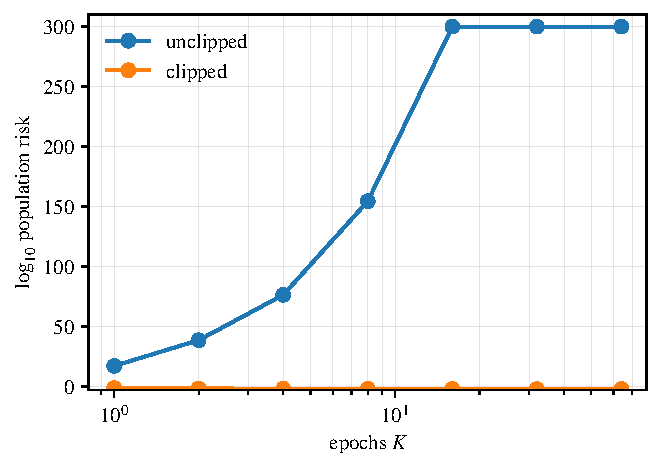
\includegraphics[width=\columnwidth]{figures/clipping_stress.pdf}
\caption{Clipping prevents instability under high coactivation and an
aggressive base step size.  Unclipped values at or above \(10^{300}\) are capped for display; subsequent updates overflow.}
\end{figure}

\section{Reproducibility}

The repository contains:

\begin{itemize}
\item \url{experiments/exact_pilots.py}, evaluating the one-hot and
singleton-filtered formulas without Monte Carlo;
\item \url{experiments/multi_active_replay.py}, generating the sparse
multi-active data and running all replay sweeps;
\item \url{experiments/plot_results.py}, recreating every paper figure;
\item checked-in CSV files and a machine-readable summary under
\url{experiments/results/}.
\end{itemize}

A quick validation takes seconds on a laptop:
\begin{verbatim}
python experiments/multi_active_replay.py
  --suite quick
\end{verbatim}
The complete checked-in sweep is reproduced with:
\begin{verbatim}
python experiments/multi_active_replay.py
  --suite full
python experiments/plot_results.py
\end{verbatim}

\end{document}
